\chapter{PyPy and RPython}
PyPy consists of two parts. 

PyPy Python Interpreter is an alterative to standard CPython implementation that aims to closely emulate behavior of CPython, written in RPython. It consists of three components: (1) bytecode compiler compiling source code of user application into Python code objects; (2) Python code objects interpreter; (3) standard object space that creates or manipulates Python objects.

RPython is a subset of Python that can be analyzed statically. The goal of RPython toolchain is to translate RPython programs into more efficient programs for various target platforms, generally ones that are considerably lower-level than Python. Compilation is carried out in the following stages:

\begin{enumerate}
\item Annotation pass performs a global analysis starting from a specified entry point inferring type of each variable and building a control flow graph. Control flow graph consists of \textit{basic blocks} that do not contain Python bytecode but rather operations after performing \textit{abstract interpretation} of the Python bytecode. Basic block always ends with jumps to other basic blocks. After construction of the flow graph has been completed, each encountered variable is annotated with the types of all possible Python objects that can be assigned to it.

\item 
The RPython Typer (or RTyper) uses the high-level information inferred during annotation phase to turn the operations in the control flow graphs into low-level operations. At this point, function inlining, \texttt{malloc} removal and other optimizations are applied. 

\item
Finally, the C backend takes flow graphs produced by \texttt{RTyper} and produces a number of C source files that are compiled into executable.
\end{enumerate}

Throughout the thesis RPython is treated as a black box. 

\section{Compile-Time Representation of RPython}

PyPltRedex works with \textbf{abstract syntax trees} and then emits RPython source code by traversing the tree and emitting strings. Abstract syntax tree itself is a tree that represent constructs of the language such as arithmetic operations, assignments, loops, etc.

In Python and other imperative languages, nodes of an abstract syntax tree can be split into two categories:

\begin{enumerate}
\item
Statements such as \texttt{while} and \texttt{for} loops, \texttt{if} statements, variable assignments.
\item
Expressions such as arithmetic operations, array element access, literal values such as integers or strings, etc.
\end{enumerate}

This allows for deeply nested expressions and can be quite tedious to work with. PyPltRedex's AST definition is modified to include \texttt{PyValue} - subset of expressions that includes only variables and literals. Expressions such as additions are thus now required to use \texttt{PyValue}, thus making resulting RPython code similar to typical three-address code intermediate representation that most compilers employ. Figure \ref{class-diagram-rpython} shows class diagram of all RPython abstract syntax tree nodes.

\begin{figure}[ht]
	\centering
	\makebox[\textwidth][c] { 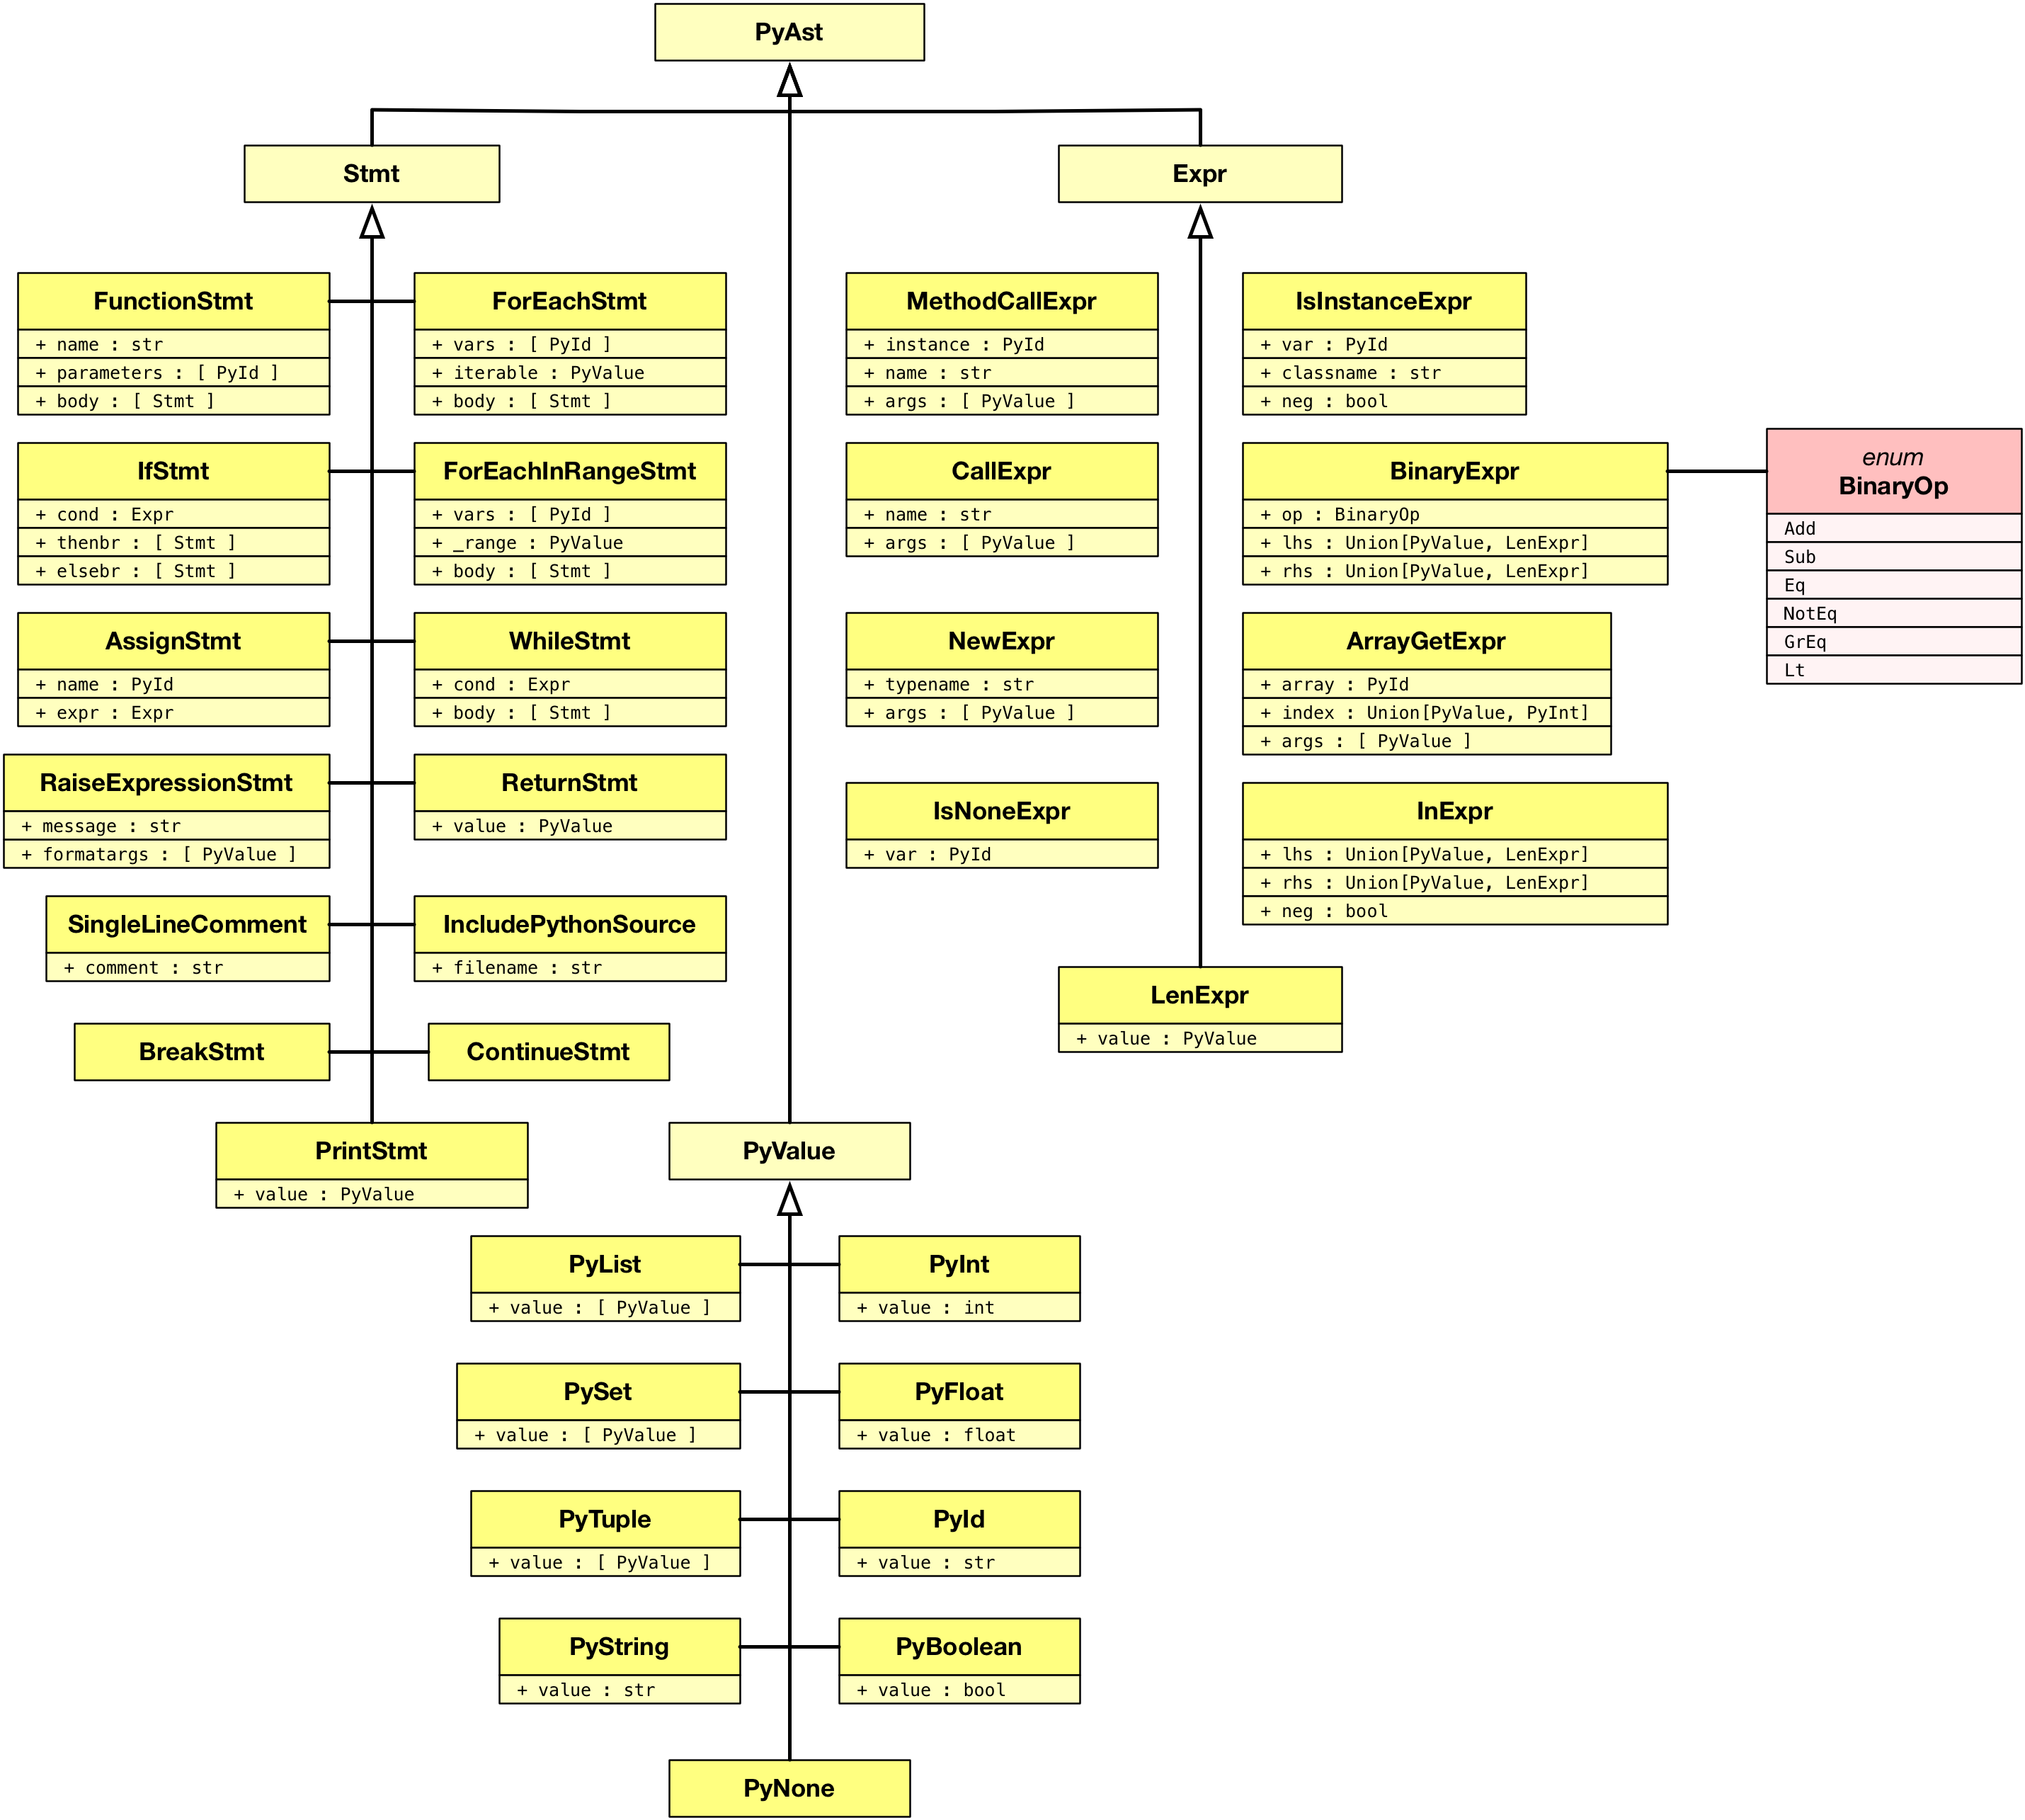
\includegraphics[scale=0.16]{class-diagram-rpython.png} }
	\caption{RPython abstract syntax tree.}
\label{class-diagram-rpython}
\end{figure}

